\chapter{Introducción}
\label{chapter:introduccion}


%%% SECTION
\section{General description of the problem}

At present, data mining processes require large amounts of data, which in many cases contain personal and private information of users or people. Although basic anonymization processes are carried out on the data, that is, elimination of names or other key identifiers, there are a multitude of re-identification techniques that allow to re-identify a user within this data set. Figure \ ref {fig: context-anoni1} presents a map where it is possible to contextualize the processes of anonymization and re-identification within a process of data mining.

\begin{figure}
	\centering
	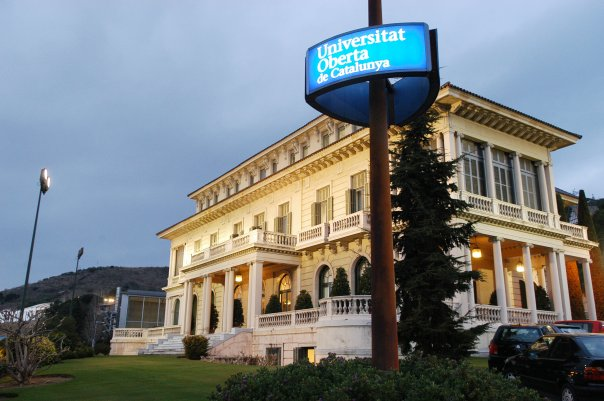
\includegraphics[width=0.6\textwidth]{figs/image1.png}
	\caption{Foot of the image.}
	\label{fig:context-anoni1}
\end{figure}

\subsection{Example of subsection}

Although important advances have been made in the preservation of privacy in the publication of data, such as the model \textit{k}-anonymity \cite{Sweeney:2002}.

An example of a pseudo-code can be found in the Code \ref{code:RandomSwitch-1}

\begin{algorithm}
	\caption{Pseudocode of the algorithm \textit{Random Switch}}
	\label{code:RandomSwitch-1}
	\begin{algorithmic}
		\REQUIRE{The original graph $ G $ and the percentage of anonymization $ p $ that you want to apply.}
		\ENSURE{El graph $G$ anonymized}
		\STATE $num = round(G.num\_edges() * p)$
		\STATE $i = 0$
		\WHILE {$i < num$}
		\STATE {$e_{1} = G.random\_edge()$}
		\STATE $e_{2} = G.random\_edge()$
		\STATE $new\_e_{1} = (e_{1}.origen, e_{2}.origen)$
		\STATE $new\_e_{2} = (e_{1}.destino, e_{2}.destino)$
		\IF {$!G.exist(new\_e_{1})$ \AND $!G.exist(new\_e_{2})$}
		\STATE $G.add\_edge(new\_e_{1})$
		\STATE $G.add\_edge(new\_e_{2})$
		\STATE $G.delete\_edge(e_{1})$
		\STATE $G.delete\_edge(e_{2})$
		\STATE $i=i+1$
		\ENDIF
		\ENDWHILE
		\RETURN $G$
	\end{algorithmic}
\end{algorithm}

An example of a table can be seen in the Table \ref{table:ejemplo_vertex_refi_query}

\begin{table}
	\centering{}
	\begin{tabular}{ l || c | c | l }
		\hline
		Node ID & $\mathcal{H}_{0}$ & $\mathcal{H}_{1}$ & $\mathcal{H}_{2}$ \\
		\hline
		\hline
		Alice & $\epsilon$ & 1 & \{4\}  \\
		\hline
		Bob & $\epsilon$ & 4 & \{1, 1, 4, 4\}  \\
		\hline
		Carol & $\epsilon$ & 1 & \{4\}  \\
		\hline
		Dave & $\epsilon$ & 4 & \{2, 4, 4, 4\}  \\
		\hline
		Ed & $\epsilon$ & 4 & \{2, 4, 4, 4\}  \\
		\hline
		Fred & $\epsilon$ & 2 & \{4, 4\}  \\
		\hline
		Greg & $\epsilon$ & 4 & \{2, 2, 4, 4\}  \\
		\hline
		Harry & $\epsilon$ & 2 & \{4, 4\}  \\
		\hline
	\end{tabular}
	\caption{\textit{Vertex refinement queries}.}
	\label{table:ejemplo_vertex_refi_query}
\end{table}